\chapter{力与平衡}
\label{Forces and equilibrium}
从本章开始是是Mechanics的内容。也就是牛顿大佬的物理学。A-Level郑重其事地把物理的内容放到数学里。真的是非常Orthodox。

\section*{学习目标}
\begin{todolist}
	\item 理解力的矢量性质,能够完成力的合成与分解
	\item 识别分析力,绘制受力分析图
	\item 掌握物体处于平衡状态时,受力为$0$
	\item 理解接触力可以分解为法向的支持力与水平方向的摩擦力
	\item 了解``光滑''模型以及限制
	\item 利用\gls{fricoeff}求算摩擦力
	\item 理解受限平衡的条件
\end{todolist}
\clearpage

\section{力的概念}
\label{sec:Force Concept}
\gls{force}是物体和物体之间的互相作用,简单理解为是一种推(排斥)或者拉(吸引)。

\subsection*{力的合成(矢量的加减法)}
\label{subsec:addition rule}
描述一个力,既需要描述大小,有需要描述力的方向,因此力就是一种\gls{vector}。既然力是矢量,那么就满足矢量的运算法则——三角形法则和平行四边形法则,如下图所示:
\begin{figure}[H]
\centering
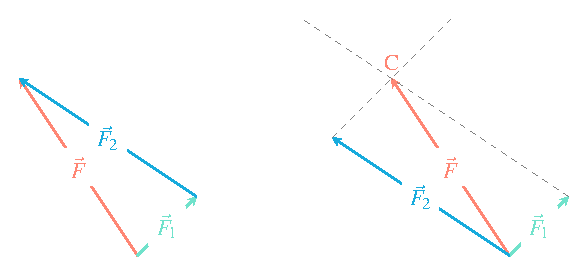
\includegraphics[width=0.8\textwidth]{trianglerule}
\caption{两个力的叠加}
\end{figure}
这就是矢量的合成。因此有$\vec{F}=\vec{F_1}+\vec{F_2}$。而矢量的减法本质上还是加法,仅需要把$\vec{F_1}-\vec{F_2}$改写成$\vec{F_1} + (-\vec{F_2})$即可。

\begin{TaskBox}
思考$-\vec{F_2}$与$\vec{F_2}$之间的关系,并利用上图绘制$\vec{F_1}-\vec{F_2}$的结果。
\end{TaskBox}

\subsection*{力的分解}
两个力既然可以通过矢量的加减法合并为一个等效的作用力,那么必然一个力也可以通过逆向过程分解为两个或者多个的作用力。一般而言我们采用正交分解,也就是建立直角坐标系,通过三角函数来描述\gls{component}的大小,通过$x$,$y$轴正方向或者负方向来描述分量的大小
\begin{figure}[H]
\centering
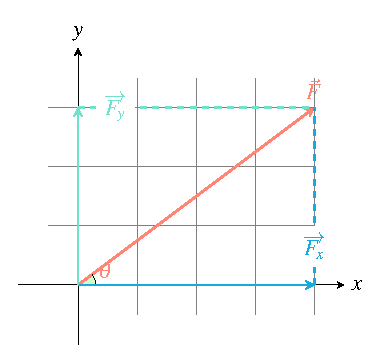
\includegraphics[width=0.8\textwidth]{decomposition}
\caption{蓝色和绿色的作用力都是红色作用力的分量}
\end{figure}

\begin{TaskBox}
根据网格,求算合力$\vec{F}$的大小,并且求算该力与$x$轴正半轴的夹角。
\tcblower
Coplanar forces, of magnitudes $F$ \si{\newton}, $3F$ \si{\newton}, $G$ \si{\newton} and $50$ \si{\newton}, act at a point $P$, as shown in the diagram.\\
\makebox{}\hfill Adapted from 2017 winter qp41 Q6
\begin{figure}[H] 
\centering
\includegraphics[width=0.5\textwidth]{resultant force}
\end{figure}
Given that $F = 0$, $G = 75$ and $\alpha = 60$\si{\degree}, find the magnitude and direction of the resultant force.
\end{TaskBox}


\subsection*{重力}
由于万有引力的作用,任何物体在地球表面上都受到地球对该物体的吸引力,这种力被称之为\gls{weight},其大小与该物体自身的质量成正比。其求算公式如下
\[
	F_G=mg
\]
$g$为比例系数,数值(在9709中)为$10$ \si{\newton\per\kg}。当然,$g$也是\gls{acdueg},是后面一章所讨论的内容。

狭义上的重力可以拓展到任意星球上,比如阿姆斯特朗,奥尔德林等$16$人都上过月球,在月球上,地球的重力就比较小了,这些航天员会受到月球表面的重力。当然由于月球质量和半径的作用,导致这种重力与他们在地球上重力力相比,只有六分之一左右。
\begin{figure}[H]
\centering
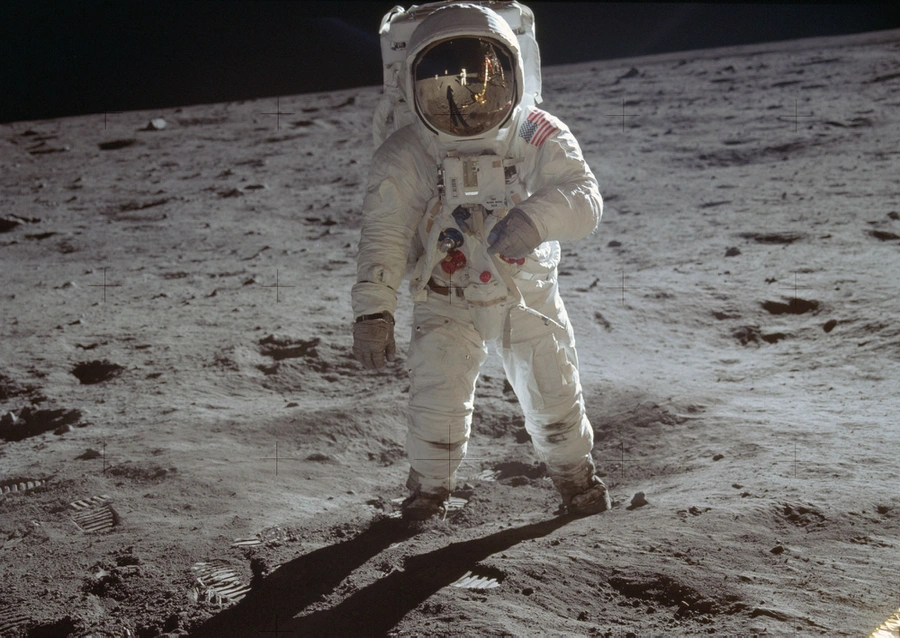
\includegraphics[width=0.4\textwidth]{Aldrin}
\caption{这张经典的照片并不是Armstrong}
\end{figure}


\subsection*{法向接触力/支持力}
%图片的位置还需要再调整。
\gls{contact}能够分解为垂直于接触面的\gls{normalf}。和水平方向的摩擦力。任何物体放在桌子上静止不动的情况下,必定有一个桌子对这些物体提供的支持力。一般计作$R$,支持力可以认为是接触粒子之间互相的排斥力导致的。
\begin{figure}[H]
\centering

\includegraphics[width=0.5\textwidth]{vase}
\caption{谁对花瓶提供了支持力?}
\end{figure}

\begin{TaskBox}
尝试标记一下桌面对花瓶的支持力
\end{TaskBox}


\subsection*{摩擦力}
当物体由于接触面产生相对运动或者运动趋势\footnote{指宏观上物体不运动}的时候。\emph{粗糙}的接触面除了提供支持力之外,还能够产生摩擦力。该摩擦力的方向总是和接触面平行,并且与相对运动或者运动趋势的方向相反。 
\begin{figure}[H]
\centering
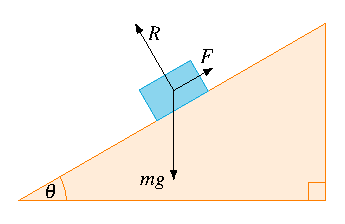
\includegraphics[width=0.5\textwidth]{inclinemodel}
\caption{物块在斜坡上静止,但是依旧有向下运动趋势}
\label{fig:inclinemodel}
\end{figure}

\subsection*{接触力}
由于支持力和摩擦力都是来自于接触面的作用力,因此用一个总的力$C$表示接触力。则有$\vec{C}=\vec{R}+\vec{F}$。并且由于摩擦力和支持力总是垂直的关系,因此
\[
	C=\sqrt{R^2+F^2}
\]

\begin{TaskBox}
尝试在上图中标记摩擦力和支持力的合力
\end{TaskBox}
\clearpage


\section{平衡状态}
\label{sec:Conditions for equilibrium}
我多么希望能够像力的平衡一样达到work-life balance啊。\\
\makebox{}\hfill 赵三金如是说

\subsection*{平衡的条件}
在\ref{fig:inclinemodel}中,如果\emph{三个力的矢量和为$0$的话},这个物块就能够保持\emph{平衡状态}。因此
\begin{definition}
When a particle is in equilibrium, the vector sum of the forces acting is zero, or equivalently, that the sum of the components in any direction is zero
\end{definition}

\subsection*{拉密定理}
\label{subsec:Lami's Theorem}
当一个物体受到三个作用力,并且作用中心都在一个点的时候,我们可以使用拉密定理\footnote{不是强制性学习内容}求算力的大小,或者两个力的夹角。拉密定理实际上是正弦定理的变形应用。
\begin{figure}[H]
\centering
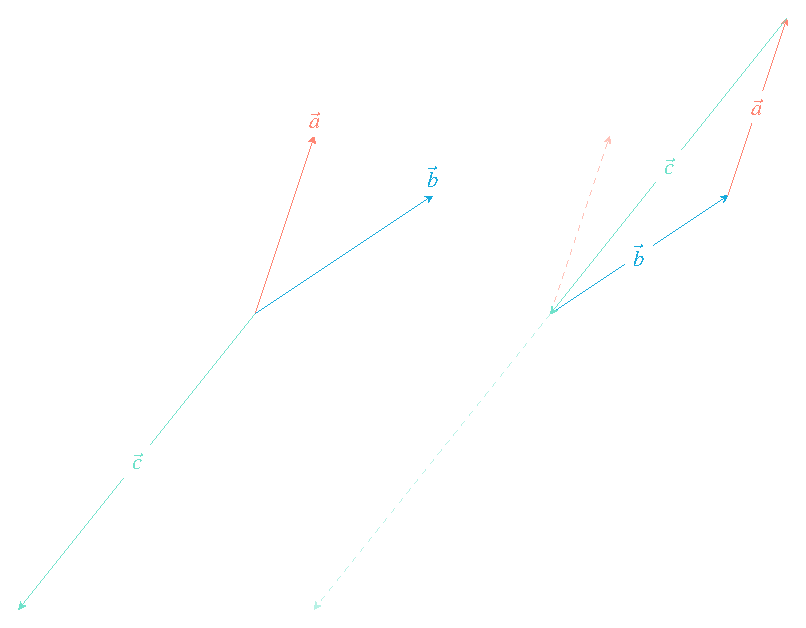
\includegraphics[width=0.8\textwidth]{lami}
\caption{三个同一起点的矢量之和为$0$可以形成首尾相接}
\label{fig:lami}
\end{figure}

\[
	\frac{\vec{a}}{\sin \alpha}=\frac{\vec{b}}{\sin \beta}=\frac{\vec{c}}{\sin \gamma}
\]
其中,$\alpha$,$\beta$,$\gamma$分别是$\vec{a}$,$\vec{b}$,$\vec{c}$所对的角

\begin{TaskBox}
在\ref{fig:lami}中标记一下$\alpha$,$\beta$,$\gamma$。并用尝试用第二张图证明。
\end{TaskBox}


\subsection*{摩擦系数}
支持力和摩擦力都是产生于物体和物体接触面之间的作用力。这两种力是紧密关联的。当物体处于相对运动时,\emph{滑动}摩擦力和支持力成正比
\[
	F=\mu R
\]
其中的$\mu$被我们称之为\gls{fricoeff}。与接触面的材料性质有关系。

\begin{figure}[H]
\centering
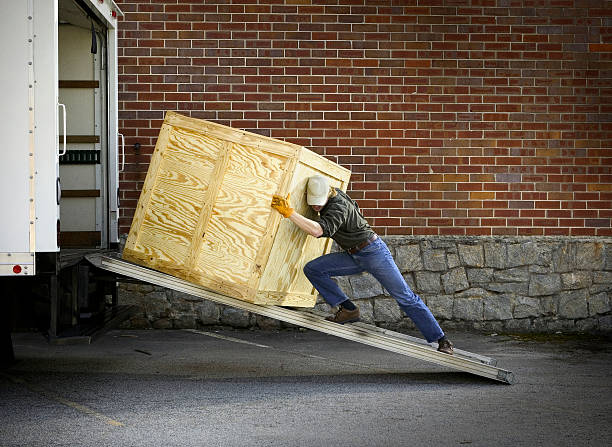
\includegraphics[width=0.8\textwidth]{pushbox}
\caption{推箱子}
\end{figure}

但是也有一些时候,箱子可能推不动,尽管人已经施加了较大的作用力。这种情况下物体仍旧处于静止状态,因而这种摩擦力被称之为\emph{静}摩擦力。静摩擦力的上限值为滑动摩擦力了。因此
\[
	F_{\text{static}} \leqslant \mu R
\]

一般而言,正常接触面的摩擦系数在,$0.3$-$0.7$之间,而我们之前所讨论的``\emph{光滑}'',其实也就是说摩擦系数为$0$,即意味着不存在任何摩擦力。

\subsection*{受限平衡}
当看到以下或者类似的描述时:
\begin{center}
about to slip\\
on the point of moving
\end{center}
这个物体到底是不是处于静止平衡的状态?这个问题的回答是肯定的。因为并没有动,但是此时是静摩擦力达到上限值了,可以直接认为通过$\mu R$进行计算。